%%%%%%%%%%%%%%%%%%%%%%%%%%%%%%%%%%%%%%%%%%%%%%%%%%%%%%%%%%%%%%%%%%%%%%
% LaTeX Example: Project Report
%
% Source: http://www.howtotex.com
%
% Feel free to distribute this example, but please keep the referral
% to howtotex.com
% Date: March 2011 
% 
%%%%%%%%%%%%%%%%%%%%%%%%%%%%%%%%%%%%%%%%%%%%%%%%%%%%%%%%%%%%%%%%%%%%%%
% How to use writeLaTeX: 
%
% You edit the source code here on the left, and the preview on the
% right shows you the result within a few seconds.
%
% Bookmark this page and share the URL with your co-authors. They can
% edit at the same time!
%
% You can upload figures, bibliographies, custom classes and
% styles using the files menu.
%
% If you're new to LaTeX, the wikibook is a great place to start:
% http://en.wikibooks.org/wiki/LaTeX
%
%%%%%%%%%%%%%%%%%%%%%%%%%%%%%%%%%%%%%%%%%%%%%%%%%%%%%%%%%%%%%%%%%%%%%%
% Edit the title below to update the display in My Documents
%\title{Project Report}
%
%%% Preamble
\documentclass[paper=a4, fontsize=11pt]{scrartcl}
\usepackage[T1]{fontenc}
\usepackage{fourier}

\usepackage[english]{babel}                                                         % English language/hyphenation
\usepackage[protrusion=true,expansion=true]{microtype}  
\usepackage{amsmath,amsfonts,amsthm} % Math packages
\usepackage[pdftex]{graphicx}   
\usepackage{epstopdf}
\epstopdfsetup{outdir=./}
\usepackage{url}
\usepackage{subfigure}


%%% Custom sectioning
\usepackage{sectsty}
\allsectionsfont{\centering \normalfont\scshape}


%%% Custom headers/footers (fancyhdr package)
\usepackage{fancyhdr}
\pagestyle{fancyplain}
\fancyhead{}                                            % No page header
\fancyfoot[L]{}                                         % Empty 
\fancyfoot[C]{}                                         % Empty
\fancyfoot[R]{\thepage}                                 % Pagenumbering
\renewcommand{\headrulewidth}{0pt}          % Remove header underlines
\renewcommand{\footrulewidth}{0pt}              % Remove footer underlines
\setlength{\headheight}{13.6pt}


%%% Equation and float numbering
\numberwithin{equation}{section}        % Equationnumbering: section.eq#
\numberwithin{figure}{section}          % Figurenumbering: section.fig#
\numberwithin{table}{section}               % Tablenumbering: section.tab#


%%% Maketitle metadata
\newcommand{\horrule}[1]{\rule{\linewidth}{#1}}     % Horizontal rule

\title{
        %\vspace{-1in}  
        \usefont{OT1}{bch}{b}{n}
        \normalfont \normalsize \textsc{} \\ [25pt]
        \horrule{0.5pt} \\[0.4cm]
        \huge Experiment Summary \\
        \horrule{2pt} \\[0.5cm]
}
\author{
        \normalfont                                 \normalsize
        Yitong Zhou (yitongz)\\[-3pt]       \normalsize
}
%\date{}

%%% Begin document
\begin{document}
\maketitle

\section{Method Summary}
\subsection{Preprocess}
I mainly implemented or used other people's source code to test with kNN, NMF, LDA and soft imputation algorithms performance on recommendations. I applied a median normalization step and denormalization step for train and test as below:
\begin{verbatim}
    % Normalzation for each row of V
    non_zero_elements = V(i,V(i, :)~=0);
    med = median(non_zero_elements);
    V(i, :) = V(i, :)/med*0.5;
    dev_med = median(abs(non_zero_elements-0.5));
    DevMed(i) = dev_med;
    if (dev_med ~= 0)
        % set the median of the deviation to the median to 0.25
        V(i, V(i, :)~=0) = 0.5+(V(i, V(i, :)~=0)-0.5)*(0.25/dev_med);
    end
    
    % Denormalzation for each row of V
    dev_med = DevMed(i);
    med = Med(i);
    % set back the median from 0.5
    b_median = median(V(i,:));
    B(i, :) = V(i, :)/b_median*med;
    non_zero_elements = B(i,B(i, :)~=0);
    b_devmedian = median(abs(non_zero_elements-med));
    if (dev_med ~= 0)
        % set back the median of the deviation from the median of 0.25
        B(i, V(i, :)~=0) = (B(i, V(i, :)~=0)-med)*(dev_med/b_devmedian)+med;
    end
\end{verbatim}

And I also used L2 normalization for kNN, soft imputation and LDA, they does not show big differences. But for NMF, L2 normalization is so bad that I have to switch to this normalization method. And for comparison purpose, all other methods are also used with median normalization.

I majorly calculated RMSE to estimate training and testing errors.
\subsection{k-Nearest Neighbour}
The kNN algorithm is quite simple: for each user, we find out k closest users and use their rating scores to estimate the scores of that user. We basically use Pearson correlation and subtract each user vector with the average to make them all center to 0.
\subsection{Nonnegative Matrix Factorization}
Other than the basic version NMF, which optimizes:
\[
	\min_{W, H} ||V-WH||_{F} \quad s.t.W, H \geq 0 
\]
I also tested with two other objective functions, which is implemented in Mandula's package (\url{https://github.com/aludnam/MATLAB/blob/master/nmfpack}).\\
Sparse NMF:
\[
	\min_{W, H} \alpha||H||_F+\sum_{i}\sum_{j} V_{ij}\log{\frac{V_{ij}}{(WH)_{ij}}-V_{ij}+(WH)_{ij}}
\]
Local NMF:
\[
	\min_{W, H}\sum_{i}\sum_{j} (V_{ij}\log{\frac{V_{ij}}{(WH)_{ij}}-V_{ij}+(WH)_{ij}) + \alpha||W^TW||_F-\beta Tr(HH^T)}
\]
I think the LNMF is based on this paper(http://www.nlpr.labs.gov.cn/users/szli/papers/Li-LNMF-ICDL-02.pdf). But I still doubt whether the SNMF is implementing the original algorithm talked about at (\url{http://www.cc.gatech.edu/~hpark/papers/GT-CSE-08-01.pdf}). My next plan is to implement these two different objective functions by myself.
\subsection{Soft Imputation}
Optimize over the objective function:
\[
	\min_{B} \frac{1}{2}||Y-B||_{F}^2 + \lambda||B||_{*}
\]
we can use proximal gradient descent to solve this problem.
\subsection{Latent Dirichilet Allocation}
The implementation of LDA is quite complicated, I used a package by Daichi Mochihahshi (\url{http://chasen.org/~daiti-m/dist/lda/}) to do the calculation. The estimation is carried out over movies, as we try to cluster movies into different topics. After training, we get two outputs:
\begin{align*}
	&\alpha = [p(t_1);p(t_2);...;p(t_k)]\\
	&\beta_i = [p(d_i|t_1);p(d_i|t_2);...;p(d_i|t_k)];\\
\end{align*}
$t_i$ is the topic i, and $d_i$ is the i-th movie. I applied the following method to estimate the ratings of a given user, movie pair:
\[ \hat{r}(u_i, t_k) = \frac{\sum_s r(u_i, d_s)p(d_s | t_k)p(t_k)}{\sum_g \sum_s  r(u_i, d_s)p(d_s | t_g)p(t_g)}\]
\[ \hat{r}(u_i, d_j) = \sum_k \hat{r}(u_i , t_k)p(d_j|t_k)\]

$\hat{r}(u_i, t_k)$ means the estimated average score for a user over a given topic.$r(u_i, d_s)$ is the observed rating data. $\hat{r}(u_i, d_j)$ is the estimated rating for a given user-movie pair.

% section a
\section{Experiment}
My current experiment covers two dataset: the Movielens dataset with 10k ratings from 1394 movies and 943 users; a pseudo dataset which still have a same dimension but with all element values as random values generated from $U[0, 1]$. 

\subsection{Pseudo Dataset}
The pseudo dataset is just a comparison against other methods. It is no surprise to see all the methods have an RMSE around 0.5 since the dataset is generated pure uniformly. However, kNN shows that it can achieve RMSE less than 0.5, which is interesting as it does show a preference over local data instead of the entire population.

\subsection{MovieLens Dataset}
The performance of all the algorithms other than kNN is really bad. kNN can reach a RMSE around 1 where all other methods can best do around 1.4. A major problem I met with is how to do normalization and renormalization correctly. Directly applying L2 norm towards NMF methods can perform really bad. The RMSE can be as large as 2 or 3. But my current rescale still does not seem to be good either, as I observed lots of predictions being too large either around 4 or 5.

Considering the fact that if we plug in row averages as the baseline, we can still get a RMSE equal to 1.06. This actually indicates that all the recommendation algorithms do not make sense in the MovieLens dataset. Metrics other than RMSE should be considered to measure the performance of these algorithms like NDCG or top ranking precisions. On the other hand, it is also possible that all these algorithms are disrupted by bad normalizations. The tricky part is without normalization, other than soft imputation, all algorithms can perform even worse. But with those normalizations, it feels like the normalization is affecting more about the result other than the methods themselves. This can be a reason why we do not see big difference between different methods.

\begin{figure}
\centering
\mbox{
\subfigure{\includegraphics[width=3in]{../../plots/V_singular_value.eps} }
}
\caption{MovieLens Dataset Singular Values} \label{fig0}
\end{figure}

Also I did a singular decomposition over the original dataset as shown in ~\ref{fig0}. The singular value seems to be exponentially distributed, which could explain that as long as we grab the mean of the datasets, it already reaches a small RMSE estimation situation.

\begin{figure}
\centering
\mbox{
\subfigure{\includegraphics[width=3in]{../../plots/knn_pseudo/uniform_rdn_rmse_knn.eps} }
\subfigure{\includegraphics[width=3in]{../../plots/soft_impute_pseudo/soft-impute-denorm_median.eps} }
}
\caption{KNN-Pseudo RMSE-k Plot and Soft Impute-Pseudo RMSE-$\lambda$ Plot} \label{fig1}
\end{figure}
\begin{figure}
\centering
\mbox{
\subfigure{\includegraphics[width=3in]{../../plots/nmf_pseudo/uniform_rdn_rmse_nmf-denorm_median_true.eps} }
\subfigure{\includegraphics[width=3in]{../../plots/nmf_pseudo/uniform_rdn_rmse_nmf.eps} }
}
\caption{NMF-Pseudo RMSE-k Plot -- Median Normalization and L2 Normalization} \label{fig2}
\end{figure}

\begin{figure}
\centering
\mbox{
\subfigure{\includegraphics[width=3in]{../../plots/knn/rmse-knn-800.eps} }
\subfigure{\includegraphics[width=3in]{../../plots/soft_impute/rmse_soft_Ymedian.eps} }
}
\caption{KNN RMSE-k Plot and Soft Impute RMSE-$\lambda$ Plot} \label{fig3}
\end{figure}
\begin{figure}
\centering
\mbox{
\subfigure{\includegraphics[width=2in]{../../plots/nmf/rmse_median_norm.eps} }
\subfigure{\includegraphics[width=2in]{../../plots/nmf/lnmf.eps} }
\subfigure{\includegraphics[width=2in]{../../plots/nmf/snmf.eps} }
}
\caption{NMF, LNMF, SNMF RMSE-k Plot} \label{fig4}
\end{figure}

\begin{figure}
\centering
\mbox{
\subfigure{\includegraphics[width=3in]{../../plots/lda/1_5_100.eps} }
\subfigure{\includegraphics[width=3in]{../../plots/lda/lda-554.eps} }
}
\caption{LDA RMSE-N Plot, $[1,100]$ and $[100, 554]$} \label{fig5}
\end{figure}

\section{Next Step}

I feel my current dilemma is that to improve the performance of collaborative filtering algorithms is very hard. One direction could be I continue my experiments in Netflix dataset which may produce good results since many people have already tried in that dataset. But the challenging part is I need to implement many algorithms in Java or C++, or at least calling them with an efficient package, since the Netflix dataset is really large, and slow algorithms like NMF can be almost impossible to be run by Matlab. Also I may consider different performance metrics. On the other hand, maybe I should focus more on NMF problems and does not necessarily focus on recommendations. I can look into image decompositions or theoretical scenarios.

\end{document}